\documentclass{cis320}
\usepackage{amssymb}
\usepackage{amsmath}
\usepackage{color}
\usepackage{mathtools}
\usepackage[linesnumbered,algoruled,boxed,lined]{algorithm2e}
\usepackage{graphicx}
\usepackage{listings}
\usepackage[makeroom]{cancel}
\graphicspath{ {./} }
\SetKwInOut{Parameter}{parameter}

\HWauthor{Zixuan Wen}{U29106598}
\HWno{1}
\HWcourse{CS 565}

%\HWextension
\newcommand\myeq{\stackrel{\mathclap{\normalfont\mbox{M.E}}}{=}}
\newcommand\myeqw{\stackrel{\mathclap{\normalfont\mbox{(10)}}}{=}}

\begin{document}
\maketitle
\HWproblem
see attached source code

\HWproblem
graph for k-means performance under different number of clusters:\\
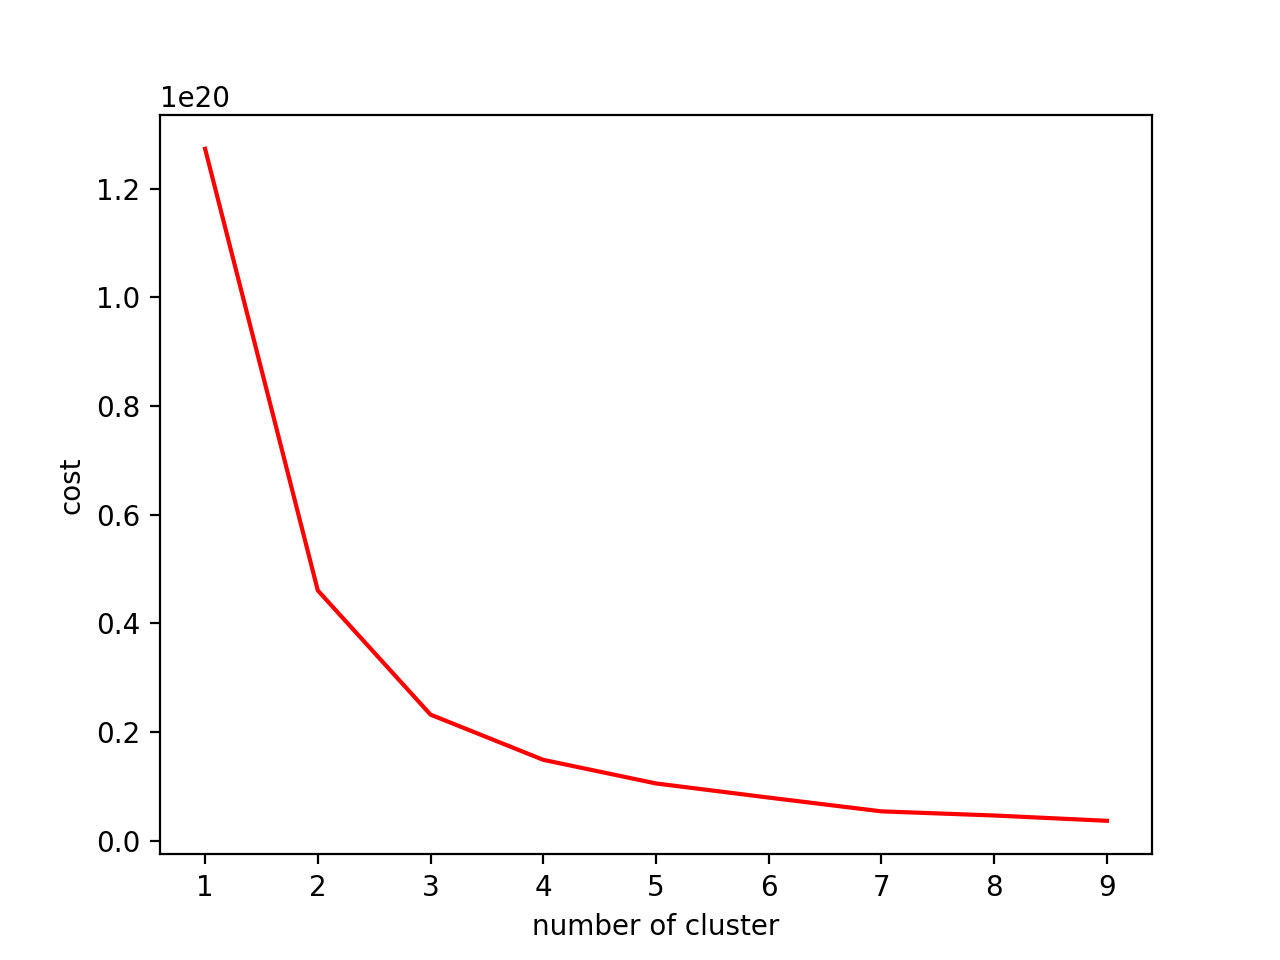
\includegraphics[width=8cm, height=6cm]{performance_k}\\
From the graph above, we can see that the cluster represents the data reasonably well when the number of cluster is around $3$ to $5$.\\
graph for k-means++ performance under different number of clusters:\\
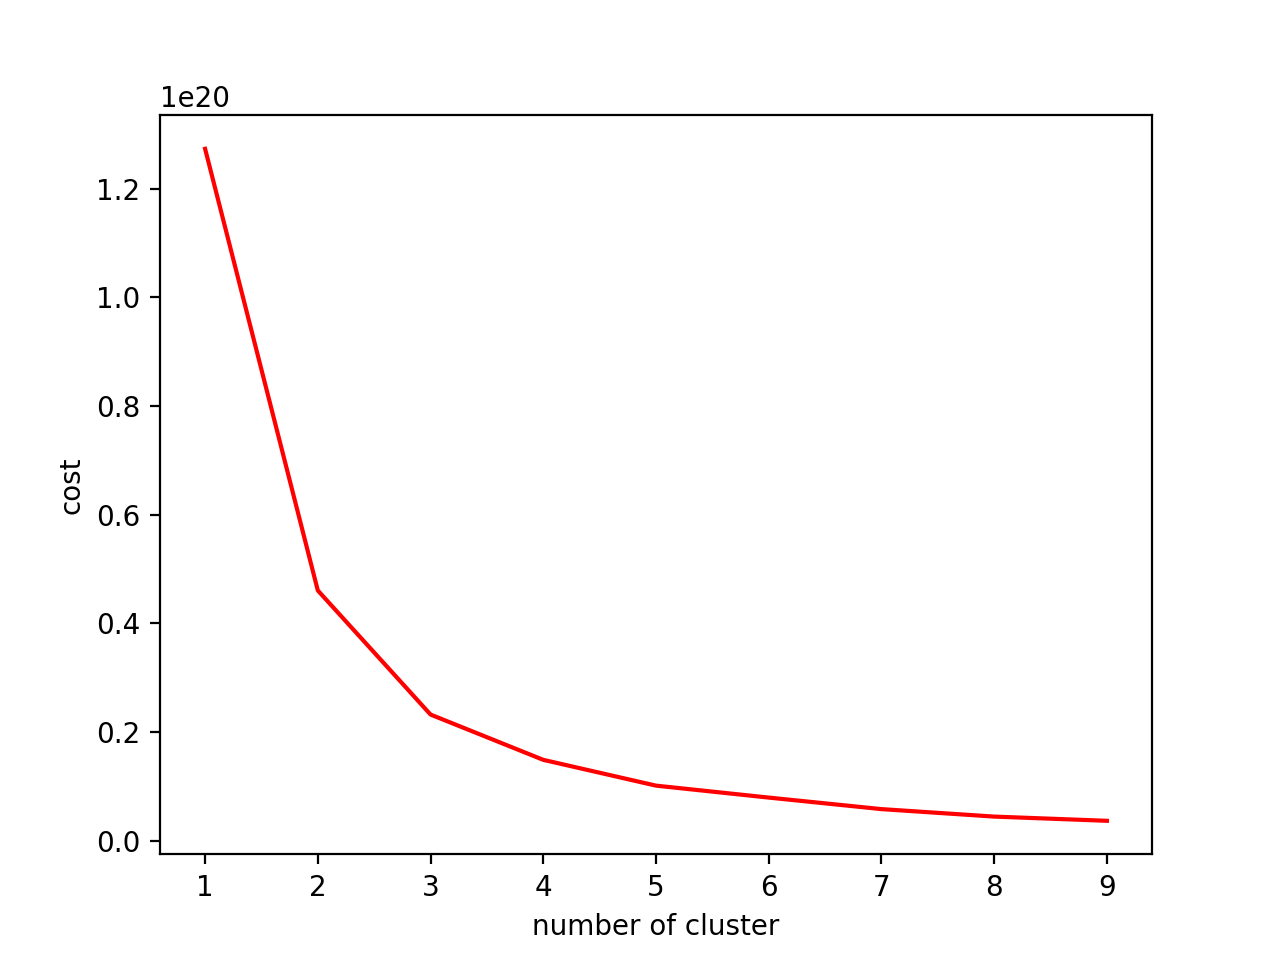
\includegraphics[width=8cm, height=6cm]{performance_k++}\\
From the graph above, we can see that the cluster represents the data reasonably well when the number of cluster is around $3$ to $5$.\\

\HWproblem
graph for cluster after PCA analyze:\\
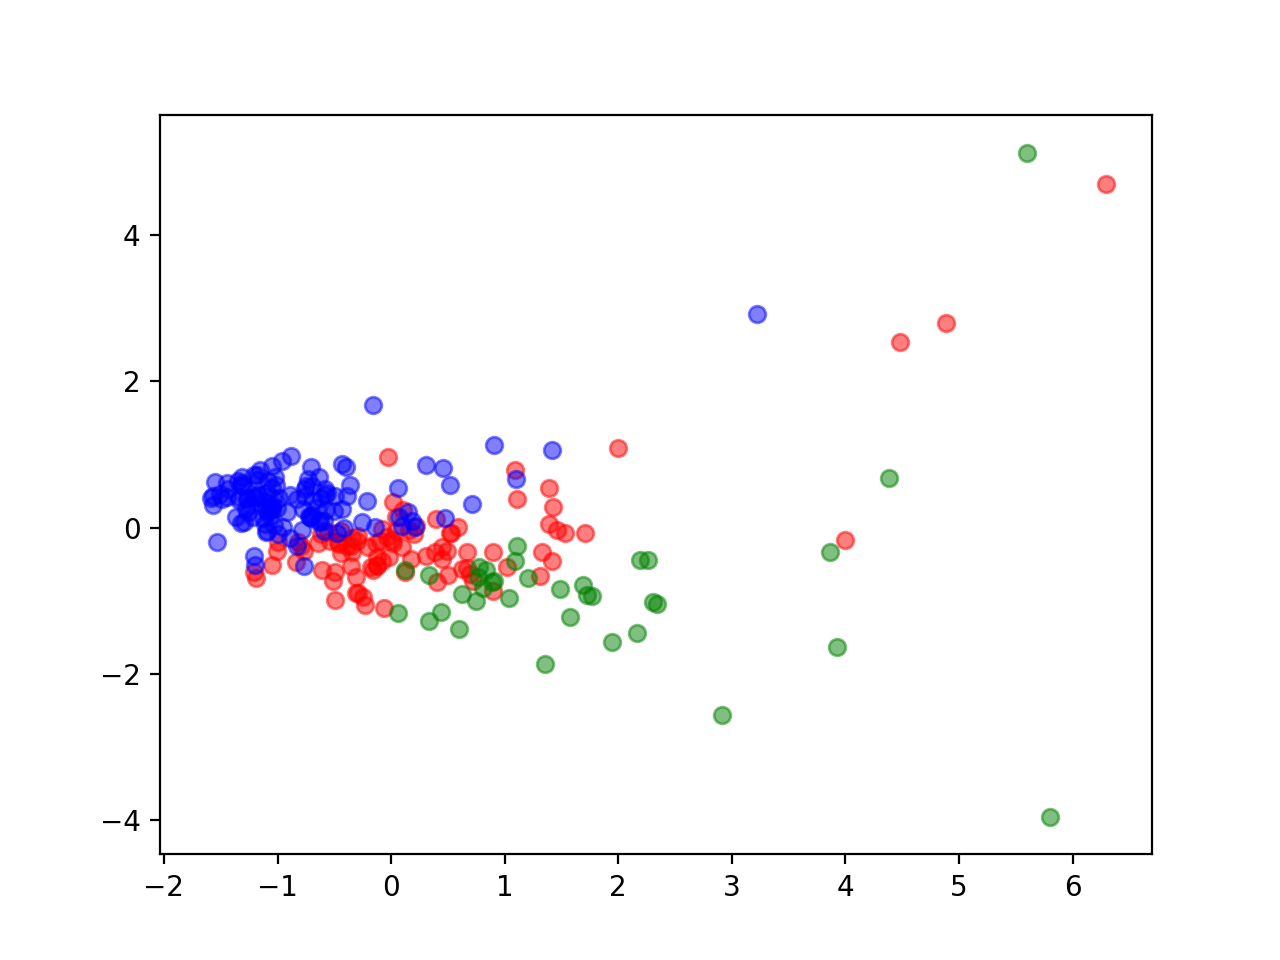
\includegraphics[width=8cm, height=6cm]{PCA_analyze}\\
From the graph above, since the data is relatively centered at the same spot due to the $total_votes$ feature, which is obtained from multiplying$ vote_average $ and $vote_count$. \\
So the cluster tend to have a long oval shape instead of regular circle one.
\HWproblem
graph for 1d-kmeans performance under different number of clusters:\\
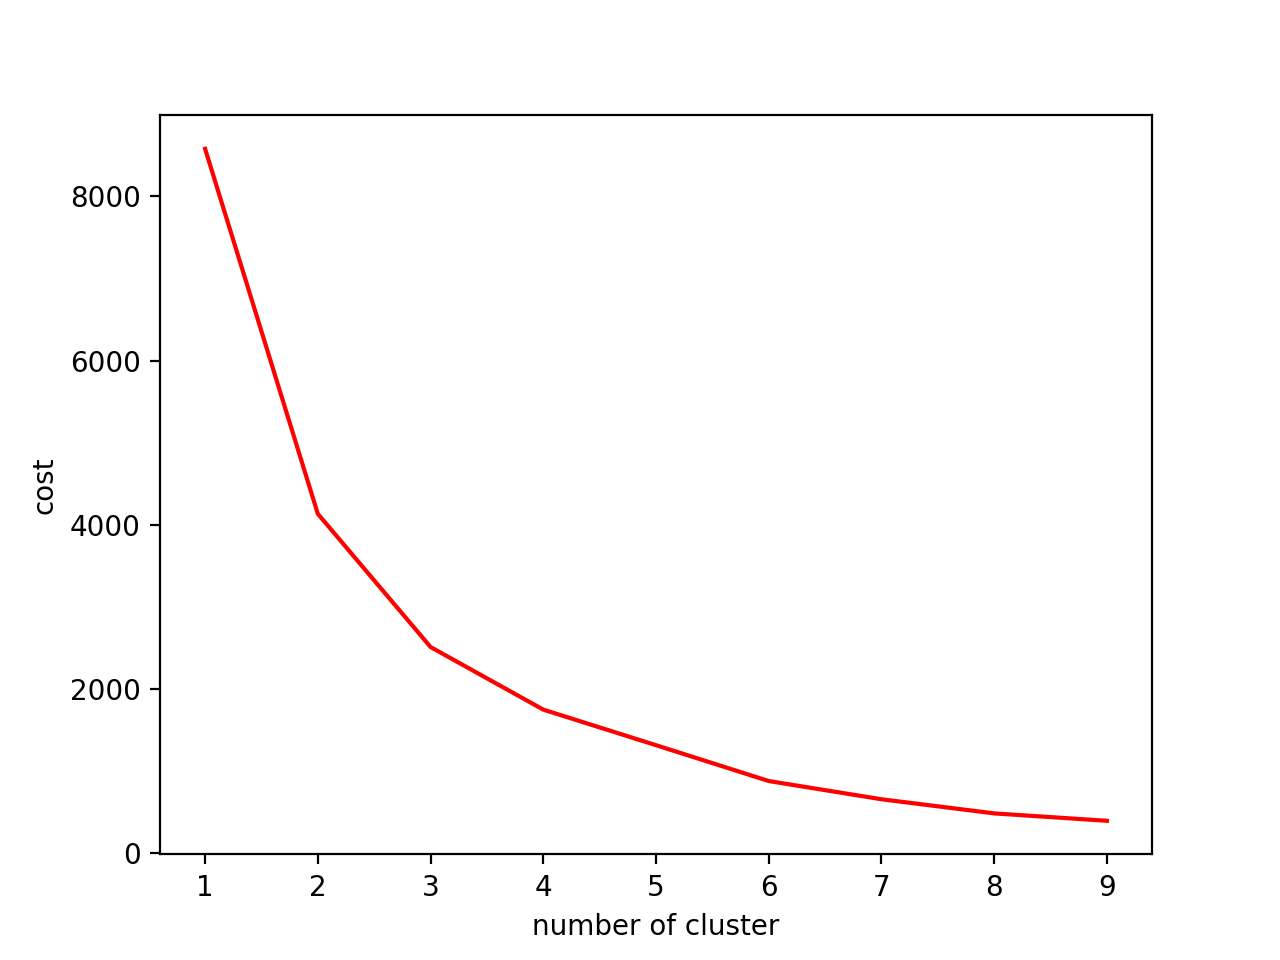
\includegraphics[width=8cm, height=6cm]{performance_1d}\\
From the graph above, we can see that the cluster represents the data reasonably well when the number of cluster is around $5$ to $7$.
\HWproblem
The computed disagreement distance of cluster produced by k-means++ and cluster produced by 1d-kmeans is $2778614$


\end{document}
